\documentclass{report}
% Include all project wide packages here.
\usepackage{fullpage}
\usepackage[style=ieee]{biblatex}
\usepackage[dutch]{babel}

\renewcommand{\familydefault}{\sfdefault}

\setmainfont[Ligatures=TeX]{Myriad Pro}
\setmathfont{Asana Math}
\setmonofont{Lucida Console}

\usepackage{titlesec, blindtext, color}
\definecolor{gray75}{gray}{0.75}
\newcommand{\hsp}{\hspace{20pt}}
\titleformat{\chapter}[hang]{\Huge\bfseries}{\thechapter\hsp\textcolor{gray75}{|}\hsp}{0pt}{\Huge\bfseries}
\renewcommand{\familydefault}{\sfdefault}
\renewcommand{\arraystretch}{1.2}
\setlength\parindent{0pt}

%For code listings
\definecolor{black}{rgb}{0,0,0}
\definecolor{browntags}{rgb}{0.65,0.1,0.1}
\definecolor{bluestrings}{rgb}{0,0,1}
\definecolor{graycomments}{rgb}{0.4,0.4,0.4}
\definecolor{redkeywords}{rgb}{1,0,0}
\definecolor{bluekeywords}{rgb}{0.13,0.13,0.8}
\definecolor{greencomments}{rgb}{0,0.5,0}
\definecolor{redstrings}{rgb}{0.9,0,0}
\definecolor{purpleidentifiers}{rgb}{0.01,0,0.01}


\lstdefinestyle{csharp}{
language=[Sharp]C,
showspaces=false,
showtabs=false,
breaklines=true,
showstringspaces=false,
breakatwhitespace=true,
escapeinside={(*@}{@*)},
columns=fullflexible,
commentstyle=\color{greencomments},
keywordstyle=\color{bluekeywords}\bfseries,
stringstyle=\color{redstrings},
identifierstyle=\color{purpleidentifiers},
basicstyle=\ttfamily\small}

\lstdefinestyle{c}{
language=C,
showspaces=false,
showtabs=false,
breaklines=true,
showstringspaces=false,
breakatwhitespace=true,
escapeinside={(*@}{@*)},
columns=fullflexible,
commentstyle=\color{greencomments},
keywordstyle=\color{bluekeywords}\bfseries,
stringstyle=\color{bluestrings},
identifierstyle=\color{purpleidentifiers}
}

\lstdefinestyle{vhdl}{
language=VHDL,
showspaces=false,
showtabs=false,
breaklines=true,
showstringspaces=false,
breakatwhitespace=true,
escapeinside={(*@}{@*)},
columns=fullflexible,
commentstyle=\color{greencomments},
keywordstyle=\color{bluekeywords}\bfseries,
stringstyle=\color{redstrings},
identifierstyle=\color{purpleidentifiers}
}

\lstdefinestyle{xaml}{
language=XML,
showspaces=false,
showtabs=false,
breaklines=true,
showstringspaces=false,
breakatwhitespace=true,
escapeinside={(*@}{@*)},
columns=fullflexible,
commentstyle=\color{greencomments},
keywordstyle=\color{redkeywords},
stringstyle=\color{bluestrings},
tagstyle=\color{browntags},
morestring=[b]",
  morecomment=[s]{<?}{?>},
  morekeywords={xmlns,version,typex:AsyncRecords,x:Arguments,x:Boolean,x:Byte,x:Char,x:Class,x:ClassAttributes,x:ClassModifier,x:Code,x:ConnectionId,x:Decimal,x:Double,x:FactoryMethod,x:FieldModifier,x:Int16,x:Int32,x:Int64,x:Key,x:Members,x:Name,x:Object,x:Property,x:Shared,x:Single,x:String,x:Subclass,x:SynchronousMode,x:TimeSpan,x:TypeArguments,x:Uid,x:Uri,x:XData,Grid.Column,Grid.ColumnSpan,Click,ClipToBounds,Content,DropDownOpened,FontSize,Foreground,Header,Height,HorizontalAlignment,HorizontalContentAlignment,IsCancel,IsDefault,IsEnabled,IsSelected,Margin,MinHeight,MinWidth,Padding,SnapsToDevicePixels,Target,TextWrapping,Title,VerticalAlignment,VerticalContentAlignment,Width,WindowStartupLocation,Binding,Mode,OneWay,xmlns:x}
}

%defaults
\lstset{
basicstyle=\ttfamily\small,
extendedchars=false,
numbers=left,
numberstyle=\ttfamily\tiny,
stepnumber=1,
tabsize=4,
numbersep=5pt
}
\addbibresource{../../library/bibliography.bib}

\title{EPO-2: Mid-term Design Report - Routeplanner in C}
\author{Robin Hes}

\begin{document}
\chapter{Systeemoverzicht}
\label{ch:systeem}
Het systeem bestaat uit drie hoofdonderdelen, de FPGA met de logica erop, de twee xBee modules voor de communicatie en het Director programma dat op de PC draait.
In figuur \ref{fig:topLevelSystem} is een blokschema van het systeem te zien, hierin is de robot nog verder opgedeeld. 
\section{Communicatie}
De communicatie tussen de robot en de director is zeer belangrijk, anders kan het doel niet bereikt worden.
De eerste versie van het communicatie protocol staat in tabel \ref{tab:comProtocol}.
Op de robot is een losse state machine geïmplementeerd (zie Figuur \ref{fig:fsmReceiver}) om de commando's onafhankelijk af te kunnen handelen en in een commando buffer te zetten, zodat het hoofd systeem deze op de correcte tijd op kan pikken.
Ook is er een losse state machine (zie Figuur \ref{fig:fsmSender}) om het versturen van een byte naar de pc af te handelen geïmplementeerd.
Beide geven een 2-bit responscode, waarvan de ene bit een response aangeeft en de andere aangeeft of de operatie succesvol was.
In Tabel \ref{tab:xBeeSettings} staan de gekozen instellingen van de xBee modules.
\begin{table}
\centering
\caption{}
\begin{subtable}{0.48\textwidth}
\subcaption{Com. Protocol Versie A}
\label{tab:comProtocol}
\centering
\begin{tabular}{|c|c|c|}
\hline
\textbf{Commando} & \textbf{hex} & \textbf{2-way} \\
\hline
Forward				& 0x46 	& to robot only\\
\hline
Stop 					& 0x53 	& to robot only\\
\hline
Right 				& 0x52 	& to robot only\\
\hline
Left 					& 0x4C 	& to robot only\\
\hline
Acknowledge 			& 0x06	& to pc only\\
\hline
Negative Acknowledge 	& 0x15	& to pc only\\
\hline
Enquiry 				& 0x05	& to pc only\\
\hline
Mine 					& 0x07	& to pc only\\
\hline
Done 				& 0x04	& to robot only\\
\hline
\end{tabular}
\end{subtable}
\quad
\begin{subtable}{0.48\textwidth}
\subcaption{xBee Settings van de twee modules. Master is de Director.}
\label{tab:xBeeSettings}
\centering
\begin{tabular}{|c|c|c|}
\hline
\textbf{Setting} & \textbf{master}& \textbf{slave} \\
\hline
Channel				& 0x1A 	& 0x1A\\
\hline
Pan ID				& 0x1337 	& 0x1337\\
\hline
Destination High			& 0x0000	& 0x0000\\
\hline
Destination Low			& 0x8564 	& 0x4658\\
\hline
My Address			& 0x4658 	& 0x8564\\
\hline
*		 			& (default)	&(default)\\
\hline
\end{tabular}
\end{subtable}
\end{table}
\begin{figure}
\centering
\caption{De FSM's op de FPGA}
\begin{subfigure}{0.23\linewidth}
\subcaption{FSM van de receiver.}
\label{fig:fsmReceiver}
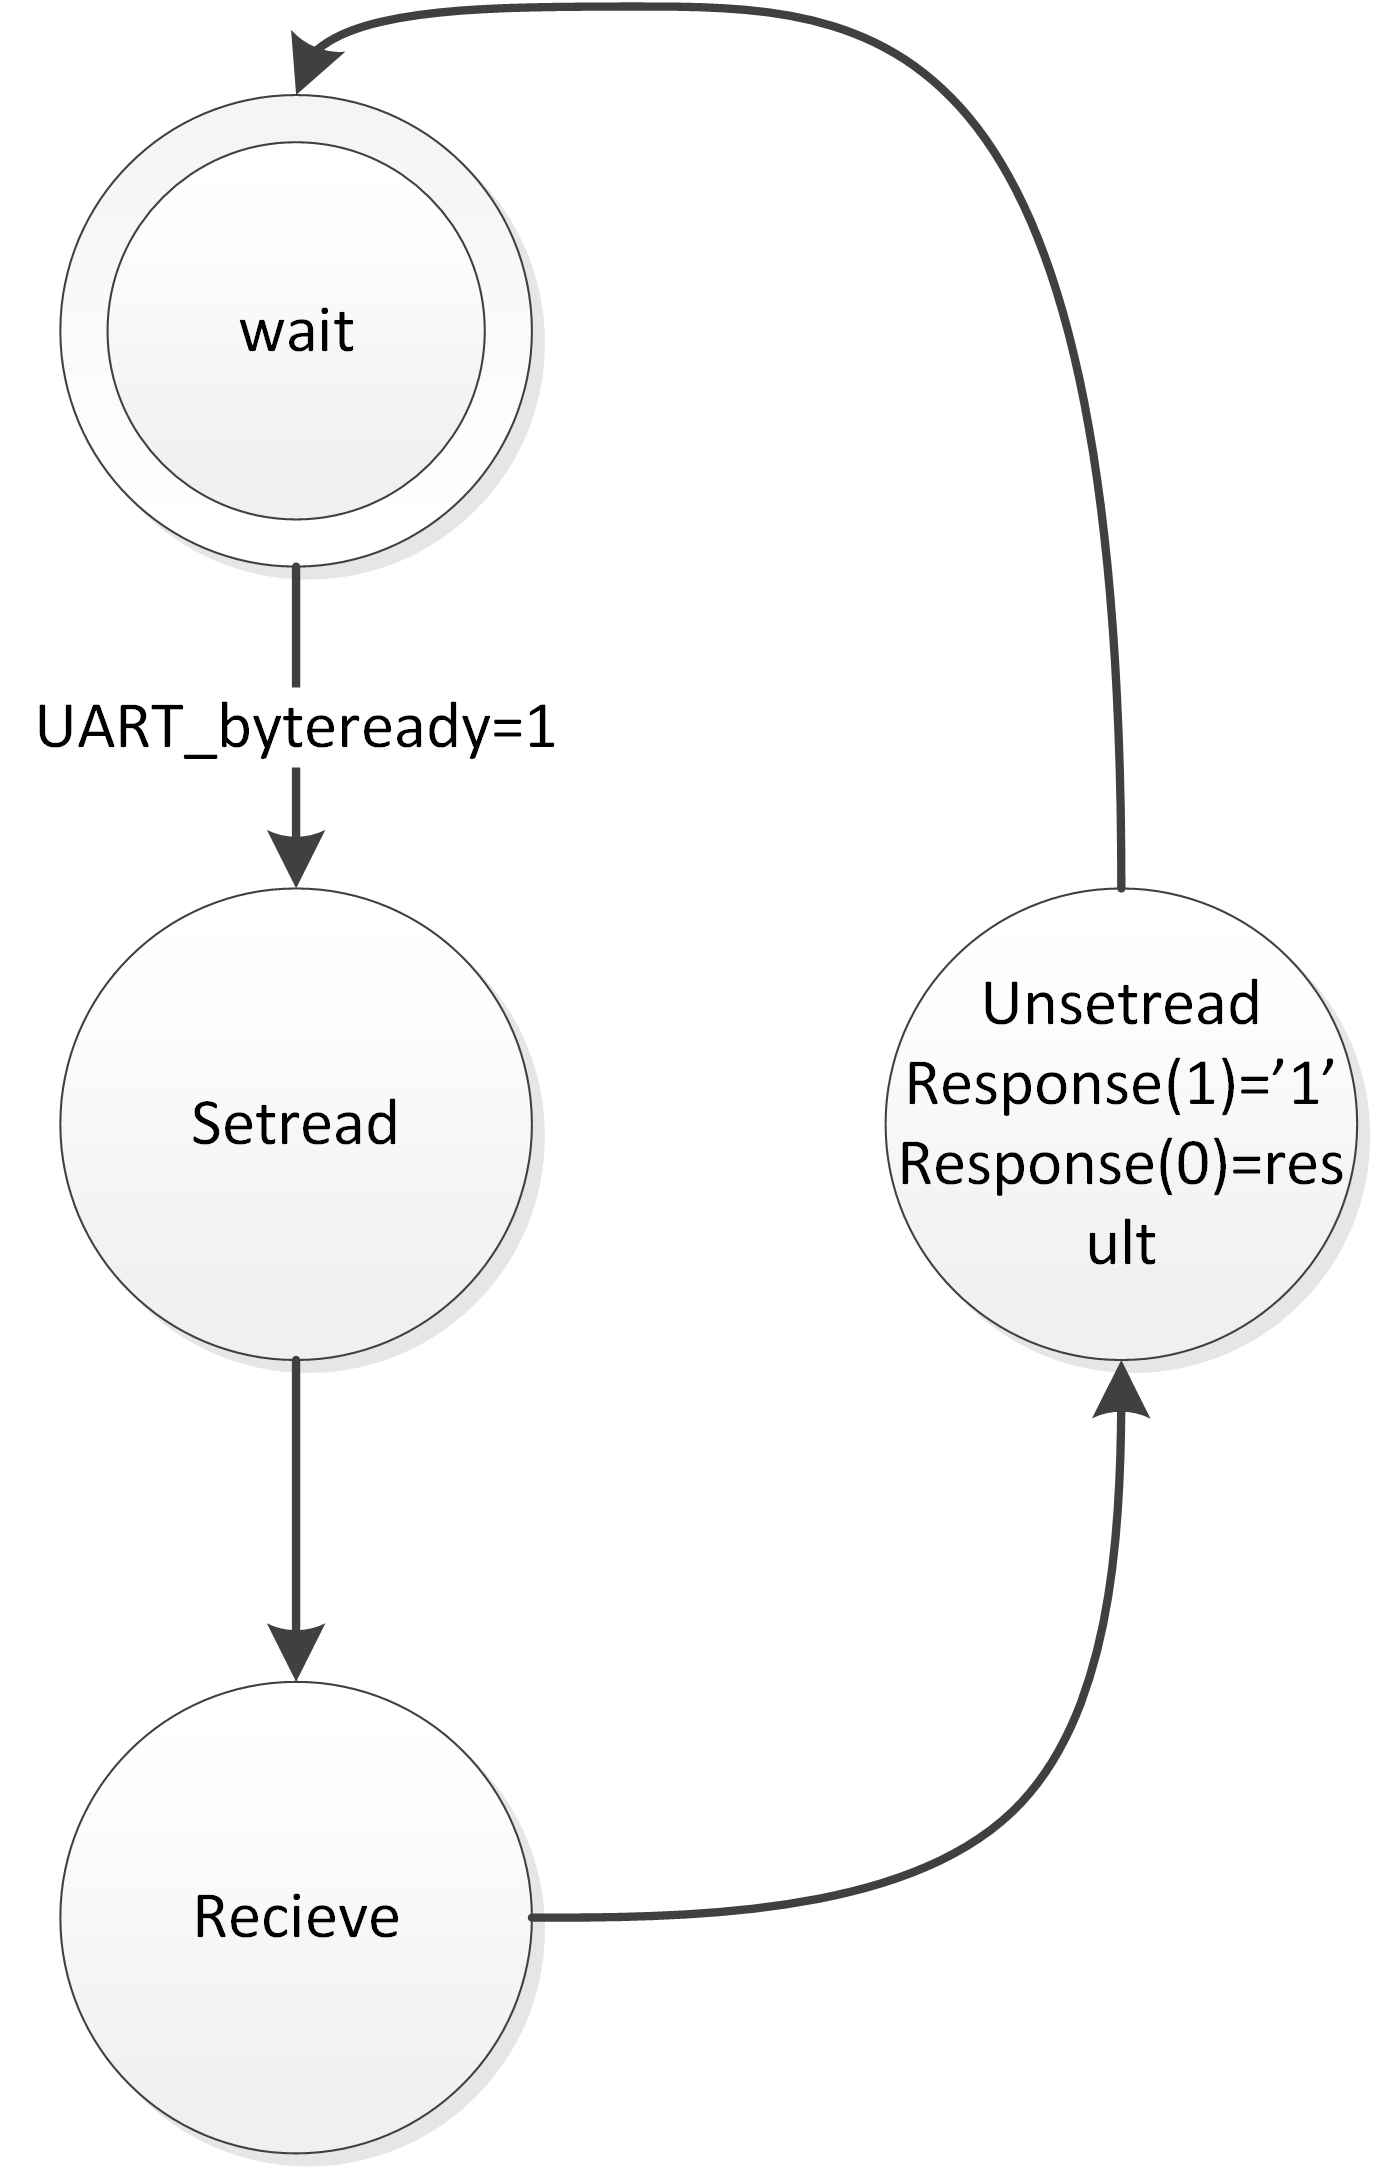
\includegraphics[width=\linewidth]{FSMReceiver}
\end{subfigure}
\quad
\begin{subfigure}{0.46\linewidth}
\subcaption{FSM van het hoofd systeem.}
\label{fig:fsmMain}
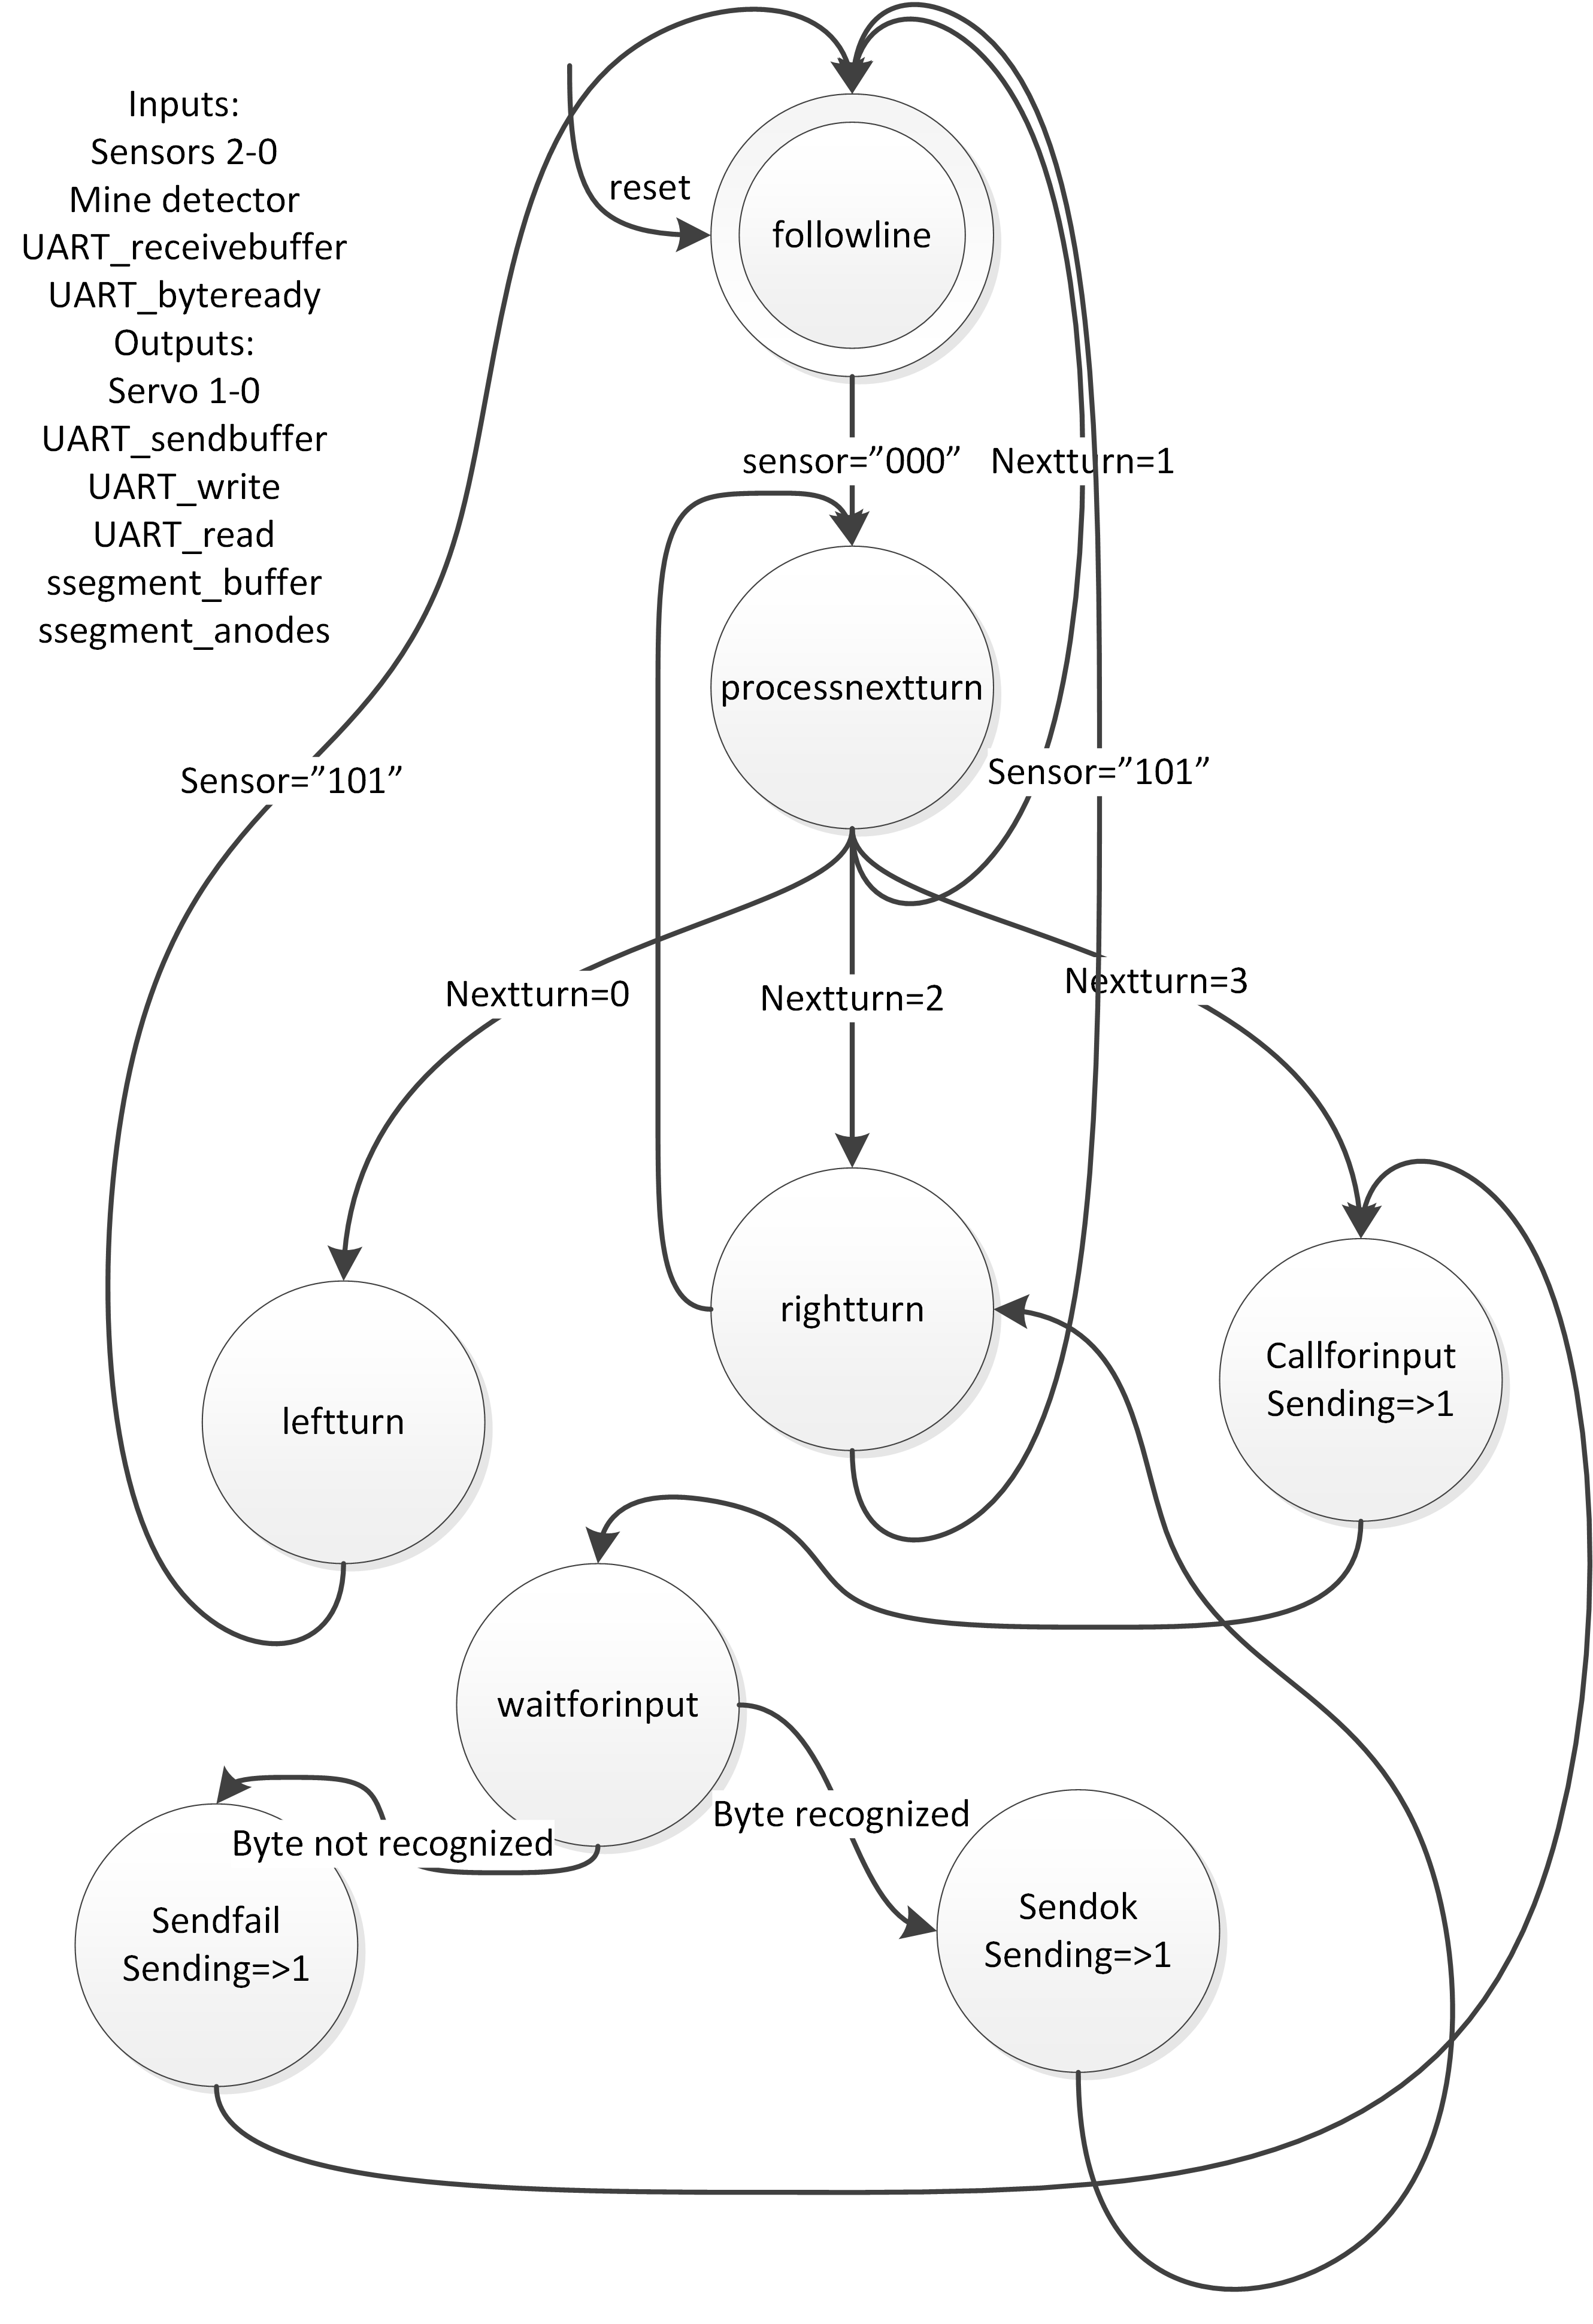
\includegraphics[width=\linewidth]{FSMMain}
\end{subfigure}
\quad
\begin{subfigure}{0.23\linewidth}
\subcaption{FSM van de sender.}
\label{fig:fsmSender}
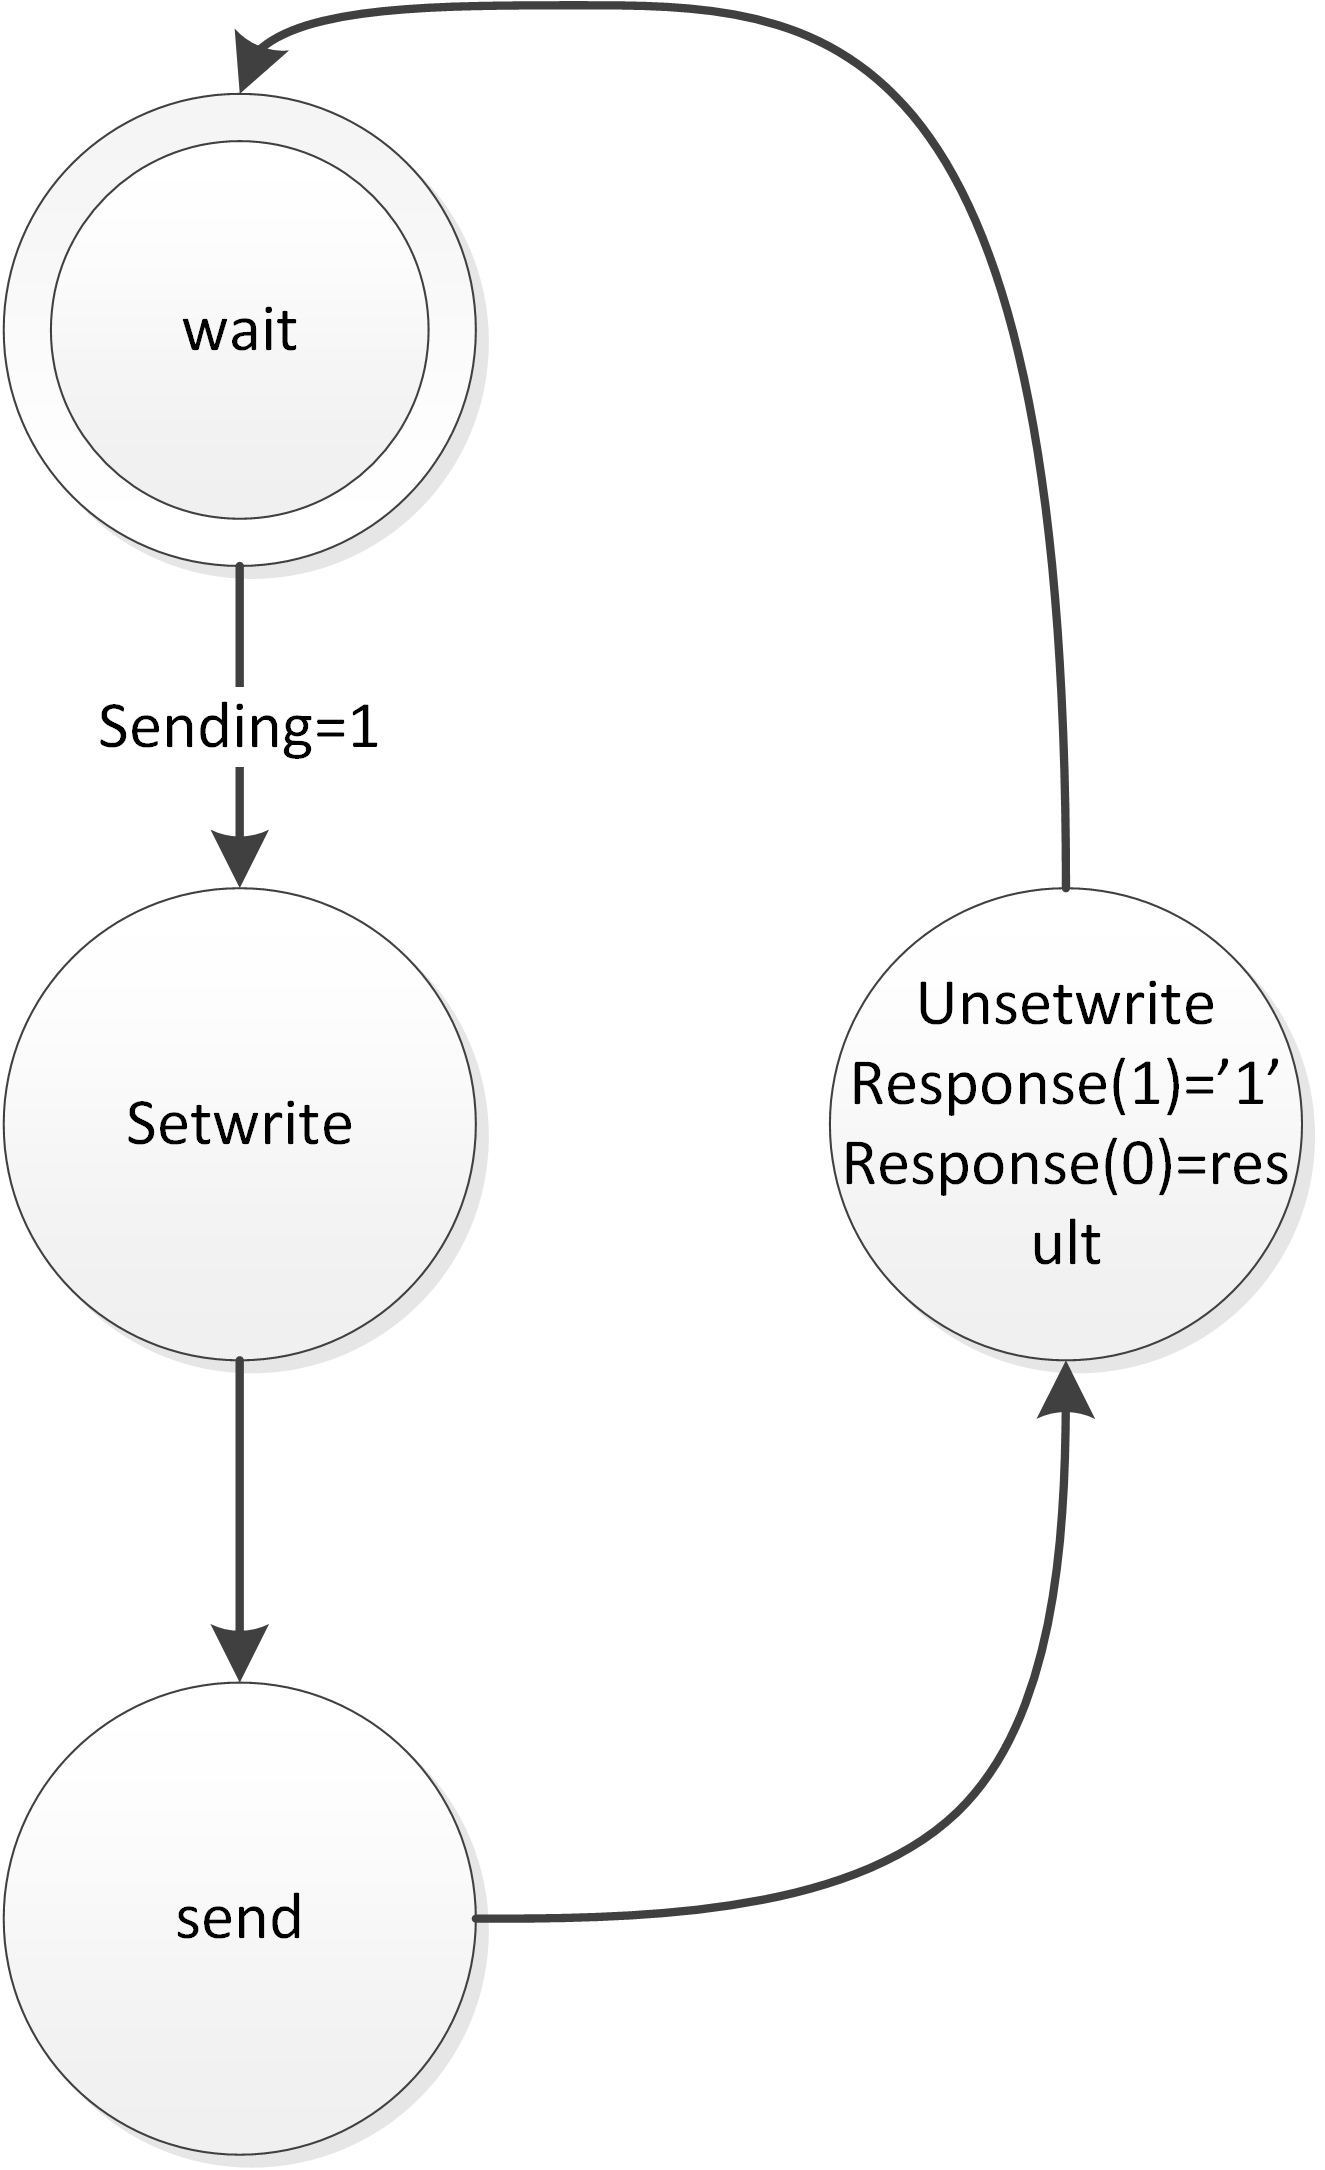
\includegraphics[width=\linewidth]{FSMSender}
\end{subfigure}
\end{figure}
\begin{figure}
\centering
\caption{Het blokschema van het Systeem.}
\label{fig:topLevelSystem}
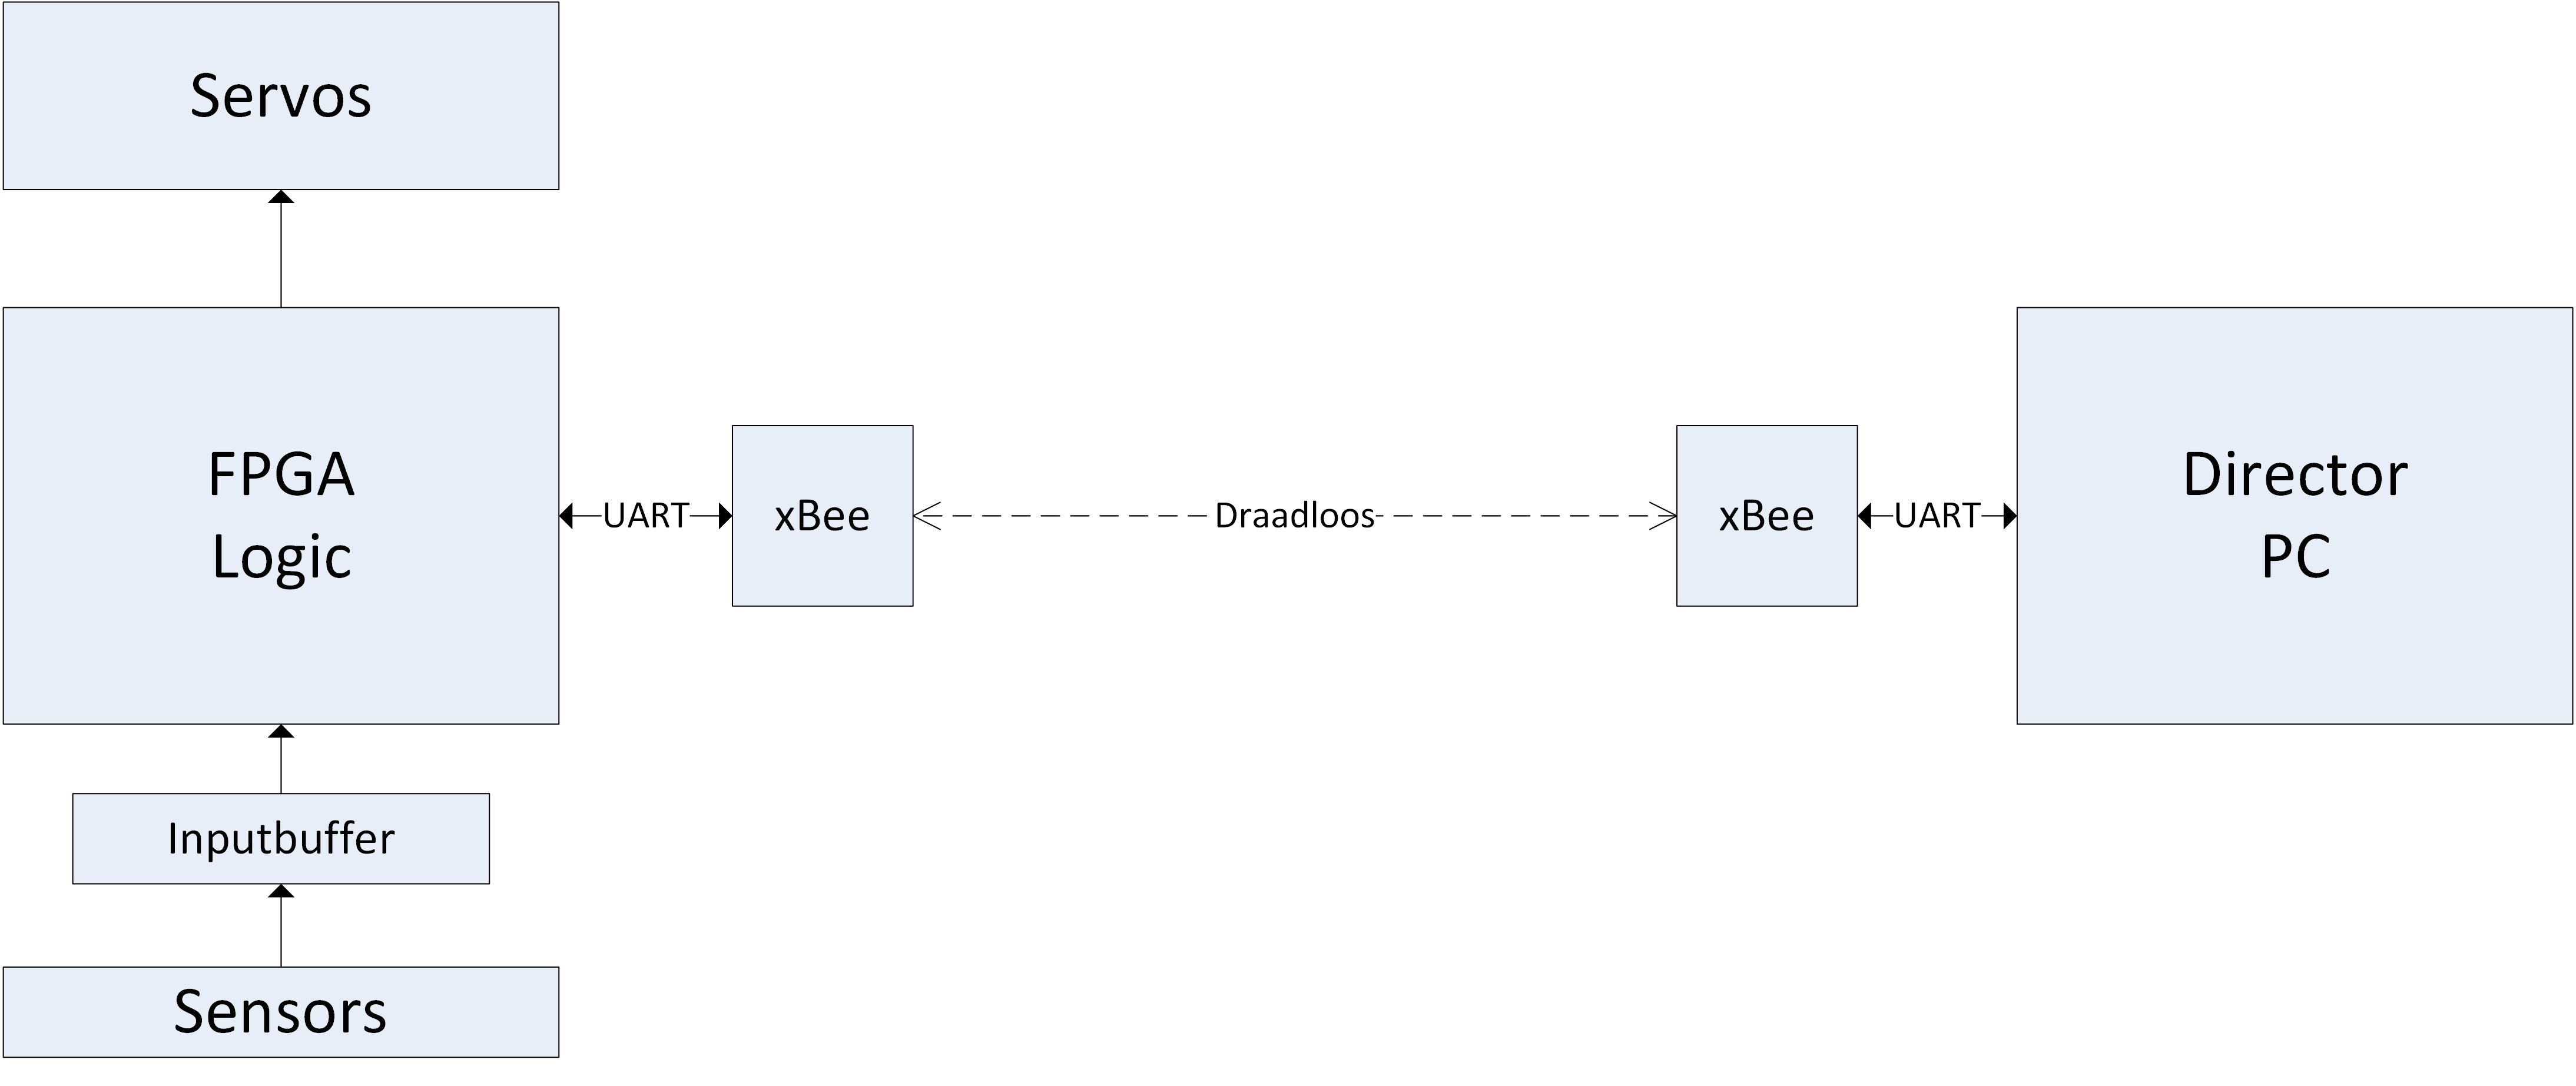
\includegraphics[width=\textwidth]{top-level-system}
\end{figure}
\section{Robot FPGA}
De FPGA handelt alle directe acties af, zoals reageren op sensoren, zodat een lijn gevolgd kan worden.
Deze stuurt ook de motoren aan, door een PWM signaal te genereren waarvan de lengte van de pulsen proportioneel is met de gekozen snelheid.
Op de FPGA wordt ook de communicatie met de xBee afgehandeld, via een UART interface.
De Finite State Machines zijn afgebeeld in de Figuren \ref{fig:fsmMain}, \ref{fig:fsmReceiver} en \ref{fig:fsmSender}.

\section{Director}
We hebben uiteindelijk, zoals te lezen is in hoofdstuk \ref{ch:route}, gekozen voor een routeplanner gebaseerd op A*. Deze compilen we naar een standaard C dll (stdcall).
Hetzelfde geldt voor de dll met de seriële interface. Deze is lichtelijk aangepast, zodat hij gemakkelijker in een andere applicatie gebruikt kan worden.
Ons hoofdproject wordt geschreven in C\# (.NET 4.5) en in combinatie met WPF (een UI framework gebaseerd op XAML UI's).
Dit geeft een vriendelijkere ontwikkelomgeving, managed talen zijn nu eenmaal wat vriendelijker voor de programmeur.
Het is ook mogelijk om alleen een van de dll's te vervangen, zodat iemand daar los aan kan werken.
Het hebben van een UI oogt prettiger en het gebruik van het eventmodel is heel fijn voor de seriële communicatie.
Dit heeft deels met persoonlijke voorkeur te maken, maar om de code voor iedereen in de projectgroep duidelijk te houden, hebben we de essentiële elementen (navigatie en communicatie) in pure C/C++ code gehouden. Al halen we misschien de seriële communicatie naar C\#, omdat je hierin een veel simpelere asynchrone afhandeling van input hebt.\\
De director moet nu nog adequaat reageren op de bytes van de robot.
Hiervoor laten we een thread constant checken of er een nieuwe byte in de input buffer zit. Zodra deze er is, geven we een event af zodat de main thread op de byte kan reageren.

\end{document}